% \documentclass[preprint]{aastex}
%\documentclass{article}
\documentclass{report}
\usepackage{graphicx}
\usepackage{subfigure}
\usepackage{rotating}
\usepackage{lscape}
\usepackage{natbib}
\usepackage{hyperref}
\pagestyle{empty}
\usepackage{aas_macros}
\usepackage{longtable}
\usepackage{amsmath}
\bibliographystyle{apj}

\hypersetup{
  bookmarks=true,         % show bookmarks bar?
  unicode=false,          % non-Latin characters in Acrobat's bookmarks
  pdftoolbar=true,        % show Acrobat's toolbar?
  pdfmenubar=true,        % show Acrobat's menu?
  pdffitwindow=true,      % page fit to window when opened
  pdftitle={Stellar Locus Regression Manual},    % title
  pdfauthor={F. William High},     % author
  pdfsubject={astronomical calibration},   % subject of the document
  pdfnewwindow=true,      % links in new window
  pdfkeywords={astronomy, colors, calibration, stars}, % list of keywords
  colorlinks=true,        % false: boxed links; true: colored links
  linkcolor=red,          % color of internal links
  citecolor=red,          % color of links to bibliography
  filecolor=magenta,      % color of file links
  urlcolor=blue           % color of external links
}

\newcommand{\zptcolor}{\boldsymbol{\kappa}}
%\newcommand{\atmextcolor}{\mathcal{E}^{\text{A}}}
%\newcommand{\galextcolor}{\mathcal{E}^{\text{G}}}
\newcommand{\atmextcolor}{\boldsymbol{E}^{\text{A}}}
\newcommand{\galextcolor}{\mathcal{E}^{\text{G}}}
%\newcommand{\color}{\mathcal{C}}
\newcommand{\color}{\boldsymbol{c}}
%\newcommand{\colormatrix}{\mathcal{M}}
\newcommand{\colormatrix}{\mathbf{B}}
\newcommand{\identity}{\boldsymbol{1}}
\newcommand{\colorairmassmatrix}{\mathbf{T}}
\newcommand{\sdss}{SDSS}
\newcommand{\slr}{SLR} 
\newcommand{\imacs}{IMACS}
\newcommand{\ldss}{LDSS3}
\newcommand{\tmass}{2MASS}
\newcommand{\reflex}{REFLEX}
\newcommand{\gof}{GOF} 
\newcommand{\ndeg}{{$^{\circ}$}}
\newcommand{\metal}{[\text{Fe}/\text{H}]}

\begin{document}

\title{Stellar Locus Regression\\User Manual}

\author{F.\ William High}

\date{\today}


\pagenumbering{roman}

%% Personalized Title Page
\begin{titlepage}
\begin{minipage}{\textwidth}
\begin{center}
\Huge
Stellar Locus Regression\\User Manual\\
\vspace{3cm}
\Large
F.~William High\\
\vspace{3cm}
\large
Department of Physics\\ Harvard
University\\ 17 Oxford Street\\ Cambridge, MA 02138\\
\href{mailto:high@physics.harvard.edu}{high@physics.harvard.edu}\\
\url{http://physics.harvard.edu/~high}
\end{center}
\end{minipage}
\end{titlepage}

\begin{minipage}{\textwidth}

\section*{}

Copyright \copyright{}  2009  Fredrick William High.\\
Permission is granted to copy, distribute and/or modify this document
under the terms of the GNU Free Documentation License, Version 1.3
or any later version published by the Free Software Foundation;
with no Invariant Sections, no Front-Cover Texts, and no Back-Cover Texts.
A copy of the license is included in the section entitled "GNU
Free Documentation License".

% \section*{Acknowledgements}

% Stellar Locus Regression was developed with Christopher Stubbs, Armin
% Rest, Brian Stalder, and Pete Challis at Harvard University.  Thanks
% to Patrick Kelly, for useful conversations.

\end{minipage}

% \begin{abstract}

%   Stellar Locus Regression (\slr) is an algorithm that takes
%   uncalibrated astronomical magnitudes of stars from any field and
%   calibrates the colors, which are magnitude differences, without the
%   traditional use of standard stars. \slr\ exploits the fact that the
%   majority of stars in the sky have colors that occupy a well defined,
%   nearly one-dimensional region in hyperdimensional color-color
%   space. This is called the stellar locus. \slr\ regresses raw colors
%   to a standard stellar locus, delivering best-fit calibration terms,
%   which can be applied to the other point- and extended-sources in the
%   catalog. \slr\ can be performed on as few as 7 stars and in fields of
%   view down to 8 arcminutes. \slr\ can be performed in real time,
%   during observation.

%   This is a short guide to installing and running the stellar locus
%   regression (\slr) on example and user data.  A more detailed
%   description of the \slr\ alogrithm and verifcation of its
%   effectiveness is available, see \citet{bib:slr}.  Since this is an
%   evolving code, this guide will supercede the paper if there are
%   differences.

% \end{abstract}


\tableofcontents
\pagenumbering{arabic}
\setcounter{page}{1}

\input{preliminaries}

\chapter{Introduction}

Stellar Locus Regression (\slr) is a method of directly adjusting the
instrumental broadband optical colors of stars to bring them into
accord with a universal stellar color-color locus, producing
accurately calibrated colors for both stars and galaxies.  

We offer an implementation of \slr\ in the Interactive Data Language
(IDL).  This manual is a guide on getting, installing, and running our
public IDL code.

The peer-reviewed paper of \citet{bib:slr} initially outlined the
broad ideas behind the technique, established the mathematical
formalism, and presented the first tests of the technique.  We expect
\slr\ to have even broader applicability to astronomy than we
envisaged in that article.

\section{What \slr\ Is}

At it's core, \slr\ simply fits instrumental colors of stars to a
standard line, delivering calibration parameters that can then be
applied to all objects in the field.

Instrumental colors are differences in instrumental magnitudes.
Instrumental magnitudes are the direct product of measuring photometry
in bias-subtracted, flat-fielded images.  Source Extractor
\citep{bib:sextractor} is the common tool for measuring instrumental
magnitudes.  The distinctive stellar locus is seen immediately in
instrumental color-color plots of stars in the field.  The red points
in the top panels of Figure \ref{fig:example} are a real example of
this.

\begin{figure}
% \epsscale{0.75}
  \center
  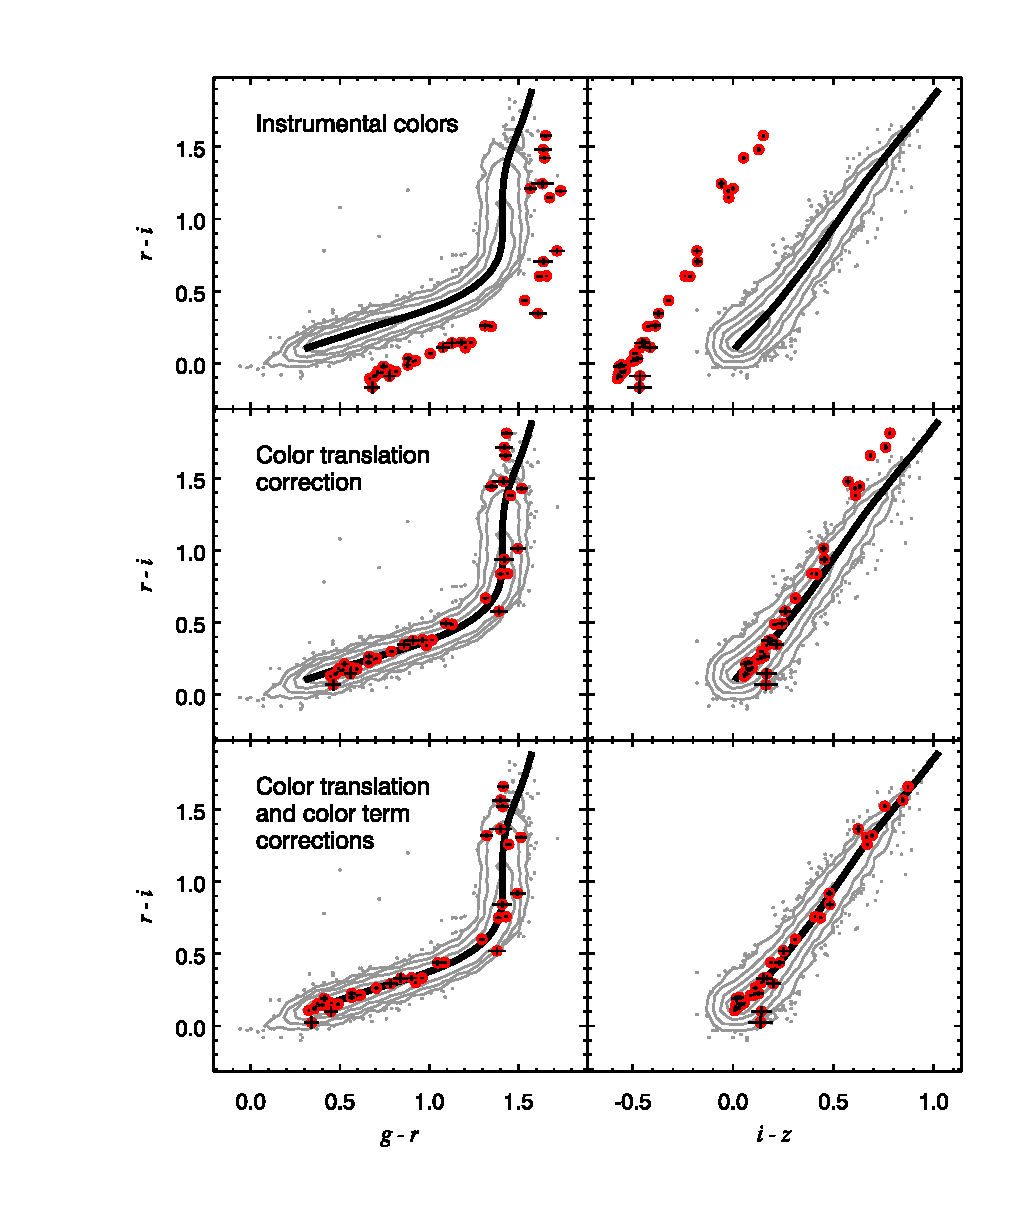
\includegraphics[scale=0.6]{fig/illus_sptcl2332_5051_locus_threepanel.eps}
  \caption{ An illustration of Stellar Locus Regression (\slr).
    Colors are plotted on the SDSS photometric system. All panels show
    the standard stellar locus (black line and gray density contours),
    reproduced from \citet{bib:covey}.  Red points are stellar colors
    obtained from a Source Extractor analysis of flat-fielded Magellan
    $6.5\,\mathrm{m}$ IMACS images.  {\it Top panels:} The
    instrumental IMACS colors are plotted, with a clear mismatch
    between them and the standard locus. {\it Middle panels:} \slr\ is
    performed with only a common translation vector applied to the
    instrumental colors.  Note the color-dependent discrepancies in
    the upper right portions of the central panels.  {\it Bottom
      panels:} Color terms are measured from a single, separate
    observation of a field containing standard stars. Fixing these
    color terms, a new best-fit translation is determined, which
    brings the observed colors onto the \sdss-calibrated color system,
    as defined by the stellar locus.  This \slr\ analysis, when the
    corrections are then applied to all objects in the photometric
    catalog, allows us to rapidly obtain highly accurate colors on the
    SDSS system, directly from flat-fielded data, with a single
    correction step that accounts for atmospheric extinction, Galactic
    extinction and instrumental response differences.}
 \label{fig:example}
\end{figure}
% \epsscale{1.0}

The instrumental stellar locus closely resembles the calibrated
stellar locus, shown with the heavy line and gray density contours in
Figure \ref{fig:example}.  If we align the two loci with simple
shifts, we arrive at the middle panels of Figure \ref{fig:example}.
The two agree somewhat, although we see a systematic difference.  This
difference arises from using a different instrument (Magellan in
Chile) than that used to make the standard stellar locus (Sloan
Digital Sky Survey telescope in New Mexico).  We measure and apply the
usual instrumental color terms, re-measure the shift, and produce a
stellar locus that matches the standard one nearly perfectly.  This is
shown in the bottom panels of Figure \ref{fig:example}.

The product is a color calibration that can be applied to all objects
in the same field where the calibrator stars appeared.  The \slr\
color calibration is achieved without first establishing individual
zeropoints for each passband, can be performed in real-time at the
telescope, and makes use of the stars from any field---they need not
be standards.  \citet{bib:slr} demonstrated how \slr\ naturally makes
one wholesale correction for differences in instrumental response, for
atmospheric transparency, for atmospheric extinction, and for Galactic
extinction.  

This all assumes that the standard locus is universal.  We explored
the extent to which this is true in \citet{bib:slr}, both in theory
and in practice.  We found that \slr\ calibrations are repeatable with
sub-percent systematic color uncertainty, that \slr\ re-calibrations
of \sdss\ data are directly sensitive to reddening by Galactic dust at
the 2\% level for the fields we looked at, and \slr\ calibrations of
red cluster galaxy colors were sufficiently accurate to deliver
cluster photometric redshifts with 0.6\% systematic uncertainty (which
we found to be consistent with 2\% color errors).

\slr\ is a simple and fundamentally different way of calibrating
photometry.  It works, and it works well.

Figure \ref{fig:algorithm} schematically outlines how \slr\ fits into
a typical calibration scheme.  The core IDL tools we have developed
are available at \url{http://stellar-locus-regression.googlecode.com},
and this manual serves as a guide to that particular code.

\begin{figure}
\center
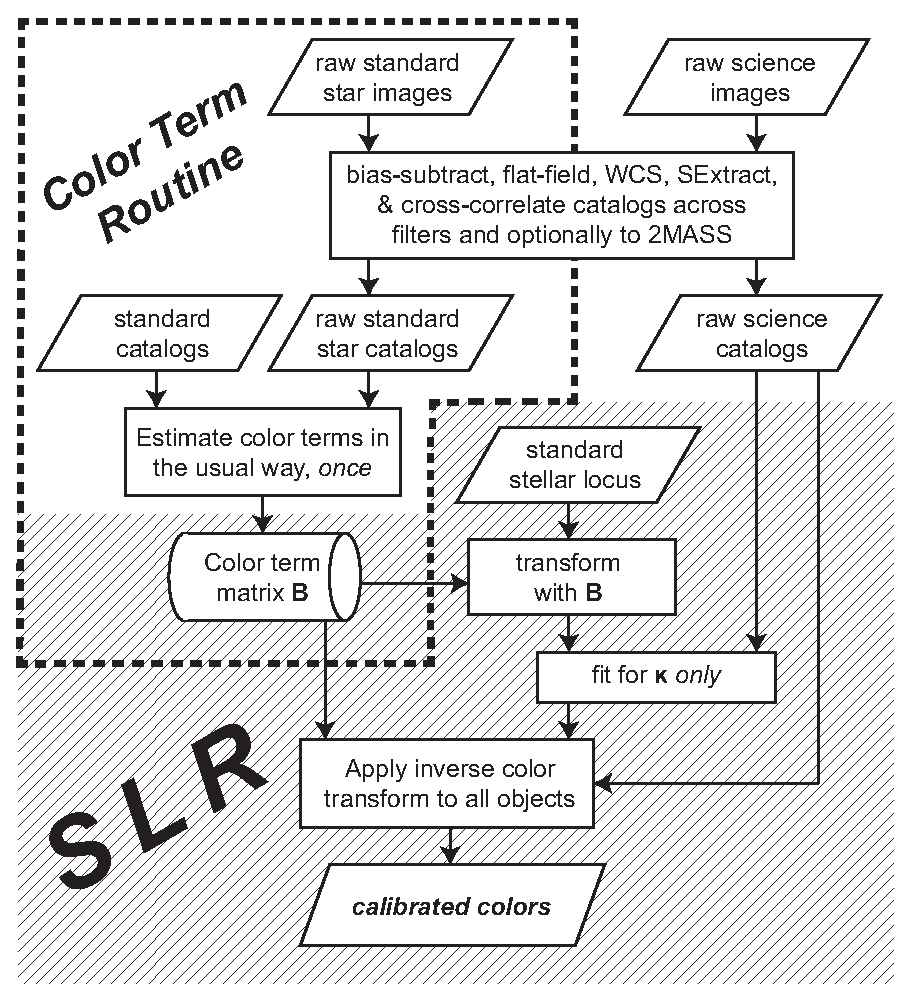
\includegraphics[scale=0.9]{fig/slr_algorithm.eps}
\caption{ \slr\ flow chart for calibrating colors.  The hashed region
  denotes parts of the algorithm that are unique to \slr, while the
  non-shaded region shows steps that are more traditional.  The dotted
  region denotes the color term estimation routine, which need only be
  performed once per detector. }
\label{fig:algorithm}
\end{figure}


\chapter{Quick Start}


\begin{enumerate}
\item \href{http://stellar-locus-regression.googlecode.com}{Download}
  the \slr\ code and unpack it in a directory of your choosing,
  $<$install-dir$>$.
\item Install and set up the \href{http://idlastro.gsfc.nasa.gov}{Goddard
    astronomy} IDL libraries,
  \href{http://www.astro.princeton.edu/~schlegel/code.html}{idlutils},
  and the \href{http://www.physics.wisc.edu/~craigm/idl}{Markwardt IDL
    libraries}.
%\item {\bf Optional:}
%  \href{http://astro.berkeley.edu/~marc/dust}{Install and set up} the
%  \citet{bib:sfd} $E(B-V)$ dust maps and IDL utilities.
\item
  \href{http://www.cfa.harvard.edu/~kcovey/research/medianlocus.tbl}{Download}
  the stellar locus data of \citet{bib:covey} and put them in a
  directory $<$data-dir$>$/covey.
\item Set environment variables (here in tcsh):
\begin{verbatim}
% setenv SLR_INSTALL <install-dir>/slr-v*
% setenv SLR_DATA <data-dir>
% setenv IDL_PATH {$IDL_PATH}:+$SLR_INSTALL/pro
% setenv PATH {$PATH}:$SLR_INSTALL/bin
\end{verbatim}
  where the version number v*\ corresponds to whatever you
  downloaded in step 1.
\item Verify your installation (see \S\ref{sec:verify}):
\begin{verbatim}
% idl
IDL> slr_docs
IDL> exit
% cd $SLR_INSTALL/example_data
% slr.csh low_reddening.ctab low_reddening.slr.ctab
% slr.csh high_reddening.ctab high_reddening.slr.ctab
% idl
IDL> slr_demo
IDL> exit
% cat low_reddening.slr.ctab
% cat low_reddening.slr
% cat high_reddening.slr.ctab
% cat high_reddening.slr
\end{verbatim}
\end{enumerate}


\chapter{Installation}

\section{Download}

First, go get the latest version 2 download at
\url{http://stellar-locus-regression.googlecode.com}. Untar
it with
\begin{verbatim}
tar xzvf slr-v*.tar.gz
\end{verbatim}
where the version number v*\ corresponds to whatever you downloaded.
Put the package in some directory $<$install-dir$>$. This can be
/usr/local/idllibraries or \$HOME or whatever you prefer. The package
root directory will then be $<$install-dir$>$/slr-v*.

Version 2.1 and higher require only IDL, and do not require
Analyst. Version 2.0 and prior require IDL with the Analyst add-on,
which costs extra.


\section{IDL Libraries}

You'll need these idl libraries:

\begin{enumerate}
\item idlutils from
  \url{http://www.astro.princeton.edu/~schlegel/code.html}.  Any
  installation procedure will do, but you probably want the latest
  idlutils tar file, e.g.\ idlutils-v5\_3\_0.tar.
\item {\it The latest} Goddard astro libraries from
  \url{http://idlastro.gsfc.nasa.gov}.  Note that idlutils comes with
  an old version of the Goddard libraries that is {\it incompatible
    with this implementation of SLR}.  Get the latest one.
\item Markwardt libraries from
  \url{http://www.physics.wisc.edu/~craigm/idl}.  You want
  cmtotal.tar.gz.
\end{enumerate}

Put them in your typical IDL directory. For example, use a directory
you can remember $<$pro-dir$>$, like /usr/local/idllibraries.

Don't forget to add them to your IDL\_PATH with shell startup file
entries similar to:
\begin{verbatim}
% export IDL_PATH=$IDL_PATH:+<pro-dir>/idlutils:+<pro-dir>/markwardt
\end{verbatim}
in bash or
\begin{verbatim}
% setenv IDL_PATH {$IDL_PATH}:+<pro-dir>/idlutils:+<pro-dir>/markwardt
\end{verbatim}
in tcsh.

Of course all of this assumes you have properly initialized the
IDL\_PATH, for example in tcsh:
\begin{verbatim}
% setenv IDL_BIN /usr/local/itt/idl/bin
% source $IDL_BIN/idl_setup
% setenv IDL_PATH <IDL_DEFAULT>
\end{verbatim}

% \section{Optional: Galactic Dust Maps}

% Some optional functionality of \slr\ requires the dust maps of
% \citet{bib:sfd}.  To enable these functions, the maps need to be
% located in \$DUST\_DIR/maps. Here's how to set this up:

% Go to \url{http://astro.berkeley.edu/~marc/dust} to get the dust maps
% and IDL code.

% Follow their install instructions. You only need the high resolution
% 4096 $E(B-V)$ maps, both the north and south Galactic planes (NGP and
% SGP). Put them in some directory, for example
% $<$install-dir$>$/slr-v2.2/example\_data/sfd/maps. Make sure the top
% directory is maps and not map. Put the SFD IDL code in some
% $<$pro-dir$>$ and add to IDL\_PATH.

% As instructed at the website, set the DUST\_DIR environment
% variable. If you used our suggestion, then you would issue
% \begin{verbatim}
% % setenv DUST_DIR <install-dir>/slr-v2.1/example_data/sfd
% \end{verbatim}

% The directory \$DUST\_DIR/maps must exist and contain the E(B-V)
% dust maps.

\section{Standard Stellar Locus}

\slr\ gets the standard stellar locus data from the directory
\$SLR\_DATA/covey.

Go get Kevin Covey's stellar locus data, which he makes available on
his own website. You'll need the stellar data\\
\url{http://www.cfa.harvard.edu/~kcovey/research/superclean.fits}\\
and the median locus line data:\\
\url{http://www.cfa.harvard.edu/~kcovey/research/medianlocus.tbl}\\
Put them in some directory $<$data-dir$>$/covey. We suggest putting
them in the $<$install-dir$>$/example\_data/covey subdirectory of
your installation. Set SLR\_DATA. If you used our suggestion, then
you would issue

\begin{verbatim}
% setenv SLR_DATA <install-dir>/example_data
\end{verbatim}

The directory \$SLR\_DATA/covey must exist and contain
medianlocus.tbl and superclean.fits.

\section{Environment Variables}

Now set some environment variables in your cshrc or bashrc file. Remember to insert the appropriate directories. Example is for tcsh:
\begin{verbatim}
% setenv SLR_INSTALL <install-dir>/slr-v1.0
% setenv SLR_DATA <data-dir>
% setenv IDL_PATH {$IDL_PATH}:+$SLR_INSTALL/pro
% setenv PATH {$PATH}:SLR_INSTALL/bin
\end{verbatim}

We've used the example directories mentioned in this install
file. This should let the demo (see below) work properly. If you made
different choices, you must make sure these environment variables
reflect them.

\chapter{Usage}
\label{sec:verify}

\section{Verifying Your Installation}

If everything is set up properly, you can run the demo by invoking IDL
and running:
\begin{verbatim}
% cd $SLR_INSTALL/example_data
% idl
IDL> slr_demo
\end{verbatim}

The first time you run it, it will take some time (it's reformatting
the data to an optimal, IDL-friendly format). It will be faster the
second time.

The demo will run \slr\ on the example Sloan Digital Sky Survey data
that comes with your installation. You should see plots of the stellar
locus (you must hit enter to continue), a visualization of the
numerical regression, and results for best-fit parameters printed to
screen.


\section{Running slr.csh Using Example Data}

Go to the directory \$SLR\_INSTALL/example\_data, then issue at
the commandline (you have to be in same directory as your input file):
\begin{verbatim}
% cd $SLR_INSTALL/example_data
% slr.csh low_reddening.ctab low_reddening.slr.ctab
\end{verbatim}

This will run \slr\ on the example colortable we provided (first
argument), and output \slr\ calibrations to another colortable (second
argument). The output colortable is equal to the input colortable but
with the additional appended columns GR, RI, etc, which are the
calibrated colors g - r, r - i. Estimated color errors, with bootstrap
errors added in quadrature, are also output.

Browse the output table of calibrated colors, and the log file that
\slr\ generates, in this case lowext\_stars3\_fwhigh.slr. The latter
contains the color calibration parameters with bootstrap errors.
\begin{verbatim}
% cat low_reddening.slr.ctab
% cat low_reddening.slr
\end{verbatim}

If that works then you should also be able to run
\begin{verbatim}
% cd $SLR_INSTALL/example_data
% slr.csh high_reddening.ctab high_reddening.slr.ctab
\end{verbatim}
Browse the output:
\begin{verbatim}
% cat high_reddening.slr.ctab
% cat high_reddening.slr
\end{verbatim}


\section{Running slr.csh with Your Own Data}

To run \slr\ on your own data, issue the command (again, in the same
directory as your input file):
\begin{verbatim}
% slr.csh input.ctab output.slr.ctab <config-file>
\end{verbatim}
The configuration file can optionally be specified.  If none is given,
then the default file is used, \$SLR\_INSTALL/config/default.config.

This has the same output as the previous section.  See
\S\ref{sec:colortable} for requirements on acceptable input colortable
formatting.

The code outputs a new colortable with calibrated colors and
optionally magnitudes, with errors.  The output filename is the input
filename with the string ``slr.ctab'' appended.  If the input filename
had ``.ctab'' as the suffix, then this suffix is first removed in
order to avoid duplication.  The \slr\ log file is the input
colortable file name with ``.slr'' appended.  Again, ``.ctab'' is
first removed if is the input file's suffix.


\section{Writing Wrappers}


At its core, \slr\ simply fits $ugrizUBVRIJHK$ colors to a standard
locus. This is done with slr\_pipe.pro.  \slr\ doesn't care where the
input magnitudes came from, nor whether they were previously
calibrated fully, partially, or at all.  \slr\ only knows how to make
the input stellar locus look like the standard locus, thereby
producing calibrated colors.

\subsection{slr\_pipe.pro}

But the real power of \slr\ comes from writing wrappers to
slr\_pipe.pro.  For example, if you have uncalibrated $griz$
magnitudes, with 2MASS $J$-band data for a subset of your stars, then
you can make a wrapper that calls slr\_pipe three times:
\begin{enumerate}
\item Calibrate only the colors $(g-r,r-i,i-z)$.  This produces the
  vector of color translations
  $\zptcolor=(\kappa_{gr},\kappa_{ri},\kappa_{iz})$.
\item Then calibrate only the colors $(i-z,z-J)$, but pass the
  calibration parameter $\kappa_{iz}$ as an input and leave it fixed
  during the fit. This produces $\kappa_{zJ}$, which happens to be
  equal to your $z$-band zeropoint (which includes atmospheric
  extinction, Galactic extinction, the instrumental zeropoint, and so
  on).
\item Run it one more time, leaving $\zptcolor$ fixed to the values
  you just measured, to produce a catalog that contains the calibrated
  colors $(g-r,r-i,i-z)$.
\end{enumerate}
All three of these tasks are within the scope of slr\_pipe, even
though they have conceptually different results.

This is made possible by passing parameters on the IDL commandline.
The best fit $\zptcolor$ can be access via the IDL keyword kappa\_out,
and its error via kappaerr\_out.  These can then be accessed then
passed to the next call of slr\_pipe using syntax like
\begin{verbatim}
IDL> slr_pipe,infile='low_reddening.ctab',$
IDL>          outfile='low_reddening.slr.ctab',$
IDL>          kappa_out=low_kappa, kapperr_out=low_kappa_err
IDL> slr_pipe,infile='low_reddening.ctab',$
IDL>          outfile='low_reddening.slr.ctab',$
IDL>          kappa_guess=low_kappa, kappa_guess_err=low_kappa_err, $
IDL>          nbootstrap=0
\end{verbatim}
In this example we've run \slr\ twice, but the second time we changed
the initial guess for $\zptcolor$ used during the regression.  We also
decided not to do the bootstrap the second time, choosing instead to
use the first bootstrap errors as our estimates for errors on the new
$\zptcolor$.

This works because any parameter that appears in the configuration
file (\S\ref{sec:config}) can be passed to slr\_pipe, verbatim.
Commandline parameters overwrite those parsed from the configuration
file.

Wrapping around slr\_pipe lets you loop over lots of data and/or run
sophisticated calibrations, like the $grizJ$ scheme described above.



\chapter{Pre-Processing Your Data}
\label{sec:prepost}

Before you run \slr, you'll have to have multiband observations of a
given field in hand.  All images must be bias-subtracted and
flat-fielded, including dome flats, fringe corrections, and ideally
illumination corrections as well.  You'll then run SExtractor or the
equivalent to detect objects in each band, and identify unique stars,
galaxies, and other objects between all bands.  The result will be a
list of instrumental magnitudes for each object in the field in each
band.  You can subtract instrumental magnitudes to arrive at
intstrumental colors.

If you want to standardize your colors to a system using a different
instrument than that originally used to establish the standard, then
you'll probably have to measure color terms, as described in
\S\ref{sec:colorterms}.

The final steps are to format your multi-band instrumental catalog
into an \slr-readable colortable \S\ref{sec:colortable}, and to tell
\slr\ about your color terms using the config files
(\S\ref{sec:config}-\ref{sec:colorterms}).  You're now ready to run
\slr.

Of course, you can also run \slr\ on photometry that has already been
calibrated to any degree.  When running \slr\ in this case, it will
give you new calibrations such that the colors resemble the standard
locus line as well as possible.






\chapter{The Colortable}
\label{sec:colortable}

SLR reads data from and outputs results to what we call {\it
  colortables}.  These are simple ascii files with a single header
that starts with \verb|#| and one row of data per object.  The header
values are columns names, and each row corresponds to one object.
Here's a simple (truncated) example:
\begin{verbatim}
# ID        RA       Dec type tmixed       g  g_err       r  r_err ...
   0 254.00649  34.33696    1      0  20.672  0.025  19.795  0.018 ...
   1 254.05269  34.36260    1      0  16.426  0.004  15.849  0.004 ...
   2 254.02026  34.34031    1      0  23.670  0.283  21.607  0.072 ...
   3 254.00436  34.36294    1      0  20.381  0.021  19.012  0.011 ...
   4 254.02655  34.34580    1      0  18.203  0.006  17.059  0.005 ...
...
\end{verbatim}
The ellipses ... here mean there can be additional columns and rows.

The columns can be any fixed width, but they must be fixed.  The
header strings however need not be fixed width.  Empty or erroneous
data must generically be represented by the character ``\verb|-|''
(dash).

While there is a minimal subset of columns that must be present for
SLR to work properly, it is acceptable for there to be extra columns
that the code doesn't formally recognize or use.  This way you can
carry extra information in the colortable, such as \verb|ID| in the
example above.

Table \ref{tab:colortable} lists the columns that are recognized and
used by the SLR code.

\begin{center}
\begin{longtable}{lllcp{2in}}
\caption[Colortable columns.]{Colortable columns.}
\label{tab:colortable} \\
  \hline \hline \\[-2ex]
  \multicolumn{1}{c}{Column name} &
  \multicolumn{1}{c}{Type} &
  \multicolumn{1}{c}{Unit} &
  \multicolumn{1}{c}{Required?} &
  \multicolumn{1}{c}{Description} \\[0.5ex] \hline
\endfirsthead
\multicolumn{5}{c}{{\tablename} \thetable{} continued: Colortable columns.} \\[0.5ex]
  \hline \hline \\[-2ex]
  \multicolumn{1}{c}{Column name} &
  \multicolumn{1}{c}{Type} &
  \multicolumn{1}{c}{Unit} &
  \multicolumn{1}{c}{Required?} &
  \multicolumn{1}{c}{Description} 
\\[0.5ex] \hline
  \\[-1.8ex]
\endhead
\multicolumn{5}{l}{{{\it Continued on next page}\ldots}} \\
\endfoot
  \\[-1.8ex] \hline \hline
\endlastfoot
\verb|ID| & {\it string} & J2000 $\deg$ & Yes & Object identifier. \\
\verb|RA| & {\it float} & J2000 $\deg$ & Yes & Right ascension. \\
\verb|Dec| & {\it float} & J2000 $\deg$ & Yes & Declination. \\
\verb|type| & {\it integer} & & Yes & $1=\textrm{star}$. Only stars should be used. If an object has a different \verb|type|, then the code will ignore it during regression, but will still apply calibrations to all objects when outputting the new colortable. \\
\verb|tmixed| & {\it boolean} & & Yes & Is the \verb|type| ambiguous between the bands? Normally you'll want to run \slr\ on unambiguous stars (\verb|tmixed| $=0$, \verb|type| $=1$). If you are low on stars in your catalog, you can try setting \verb|tmixed| to 1, in which case \slr\ will use all objects of the specified \verb|type|. \\
\verb|U| & {\it float} & mag & UNTESTED & $U$-band magnitude. \\
\verb|U_err| & {\it float} & mag & If \verb|U| present & Uncertainty in Johnson $U$-band magnitude. \\
\verb|B| & {\it float} & mag & UNTESTED & $B$-band magnitude. \\
\verb|B_err| & {\it float} & mag & If \verb|B| present & Uncertainty in Johnson $B$-band magnitude. \\
\verb|V| & {\it float} & mag & UNTESTED & $V$-band magnitude. \\
\verb|V_err| & {\it float} & mag & If \verb|V| present & Uncertainty in Johnson $V$-band magnitude. \\
\verb|R| & {\it float} & mag & UNTESTED & $R$-band magnitude. \\
\verb|R_err| & {\it float} & mag & If \verb|R| present & Uncertainty in Johnson $R$-band magnitude. \\
\verb|I| & {\it float} & mag & UNTESTED & $I$-band magnitude. \\
\verb|I_err| & {\it float} & mag & If \verb|I| present & Uncertainty in Johnson $I$-band magnitude. \\
\verb|u| & {\it float} & mag & UNTESTED & $u$-band magnitude. \\
\verb|u_err| & {\it float} & mag & If \verb|u| present & Uncertainty in SDSS $u$-band magnitude. \\
\verb|g| & {\it float} & mag & No & $g$-band magnitude. \\
\verb|g_err| & {\it float} & mag & If \verb|g| present & Uncertainty in SDSS $g$-band magnitude. \\
\verb|r| & {\it float} & mag & No & $r$-band magnitude. \\
\verb|r_err| & {\it float} & mag & If \verb|r| present & Uncertainty in SDSS $r$-band magnitude. \\
\verb|i| & {\it float} & mag & No & $i$-band magnitude. \\
\verb|i_err| & {\it float} & mag & If \verb|i| present & Uncertainty in SDSS $i$-band magnitude. \\
\verb|z| & {\it float} & mag & No & $z$-band magnitude. \\
\verb|z_err| & {\it float} & mag & If \verb|z| present & Uncertainty in SDSS $z$-band magnitude. \\
\verb|J| & {\it float} & mag & No & $J$-band magnitude. \\
\verb|J_err| & {\it float} & mag & If \verb|J| present & Uncertainty in SDSS $J$-band magnitude. \\
\verb|H| & {\it float} & mag & UNTESTED & $H$-band magnitude. \\
\verb|H_err| & {\it float} & mag & If \verb|H| present & Uncertainty in SDSS $H$-band magnitude. \\
\verb|K| & {\it float} & mag & UNTESTED & $K$-band magnitude. \\
\verb|K_err| & {\it float} & mag & If \verb|K| present & Uncertainty in SDSS $K$-band magnitude. \\
\end{longtable}
\end{center}







\chapter{Configuration Parameters}
\label{sec:config}

SLR reads ascii configuration files that the user can edit.  Comments
can be used with the character \verb|#|.  There must be at least one
space between the parameter name and its value.  Arrays (vectors) are
comma-separated lists; there must be no spaces in such lists.  Each
parameter in the config file must have a corresponding value next to
it.  There can be no empty fields.  All parameters must be present in
the file.

Table \ref{tab:config} describes all configuration paramaters.

\begin{center}
\begin{longtable}{llp{2in}}
\caption[Configuration parameters.]{Configuration parameters.}
\label{tab:config} \\
  \hline \hline \\[-2ex]
  \multicolumn{1}{c}{Parameter} &
  \multicolumn{1}{c}{Type} &
  \multicolumn{1}{c}{Description} \\[0.5ex] \hline
\endfirsthead
\multicolumn{3}{c}{{\tablename} \thetable{} continued: Configuration parameters.} \\[0.5ex]
  \hline \hline \\[-2ex]
  \multicolumn{1}{c}{Parameter} &
  \multicolumn{1}{c}{Type} &
  \multicolumn{1}{c}{Description} 
\\[0.5ex] \hline
  \\[-1.8ex]
\endhead
\multicolumn{3}{l}{{{\it Continued on next page}\ldots}} \\
\endfoot
  \\[-1.8ex] \hline \hline
\endlastfoot

~ & ~ & ~ \\ \hline
\multicolumn{3}{c}{Colors to calibrate} \\
\hline ~ & ~ & ~ \\ 

\verb|colors2calibrate| & {\it string array} & Colors to be calibrate by SLR. Comma separated list, eg, \verb|gr,ri,iz,zJ| \\
\verb|kappa_fix| & {\it boolean array} & Fix $\zptcolor$? There must be one entry for each \verb|colors2calibrate|. Can be mixed, eg, \verb|1,0,0,0|. \\
\verb|kappa_guess| & {\it float array} & {\it Initial} values of $\zptcolor$ for the fitting routine whenever \verb|kappa_fix| is 0, or {\it fixed} values of $\mathbf{\kappa}$ whenever \verb|kappa_fix| is 1. In magnitudes. There must be one entry for each \verb|colors2calibrate|. \\
\verb|kappa_guess_err| & {\it float array} & Values of errors for $\zptcolor$, used when not bootstrapping or when only transforming the colors. In magnitudes. \\
\verb|kappa_guess_range| & {\it float array} & Range of acceptable values of $\zptcolor$, used by the fitting routine. In magnitudes. There must be one entry for each \verb|colors2calibrate|. \\

~ & ~ & ~ \\ \hline
\multicolumn{3}{c}{Color terms} \\
\hline ~ & ~ & ~ \\ 

\verb|colorterms| & {\it float array} & Color terms to use. \\
\verb|colortermbands| & {\it string array} & Comma separated list of the bands that use the color terms. Each band here must appear somewhere in \verb|colors2calibrate|, although not all magntiudes in \verb|colors2calibrate| need have a \verb|colortermband|.  See \S\ref{sec:colorterms}.  If {\tt none}, then color terms are not used. \\
\verb|colormult| & {\it string array} & Comma separated list of the colors that multiply the \verb|colorterms|. \\

~ & ~ & ~ \\ \hline
\multicolumn{3}{c}{Controlling the fitter} \\
\hline ~ & ~ & ~ \\ 

\verb|transform_only| & {\it boolean} & If yes, then don't do regression and just calibrate the data using the input $\zptcolor$ and colorterms.  If no, fit for $\zptcolor$ and then perform the color transformation. \\
\verb|weighted_residual| & {\it boolean} & Use the error-weighted residual? \\
\verb|nbootstrap| & {\it integer} & Number of bootstraps to perform. \\

~ & ~ & ~ \\ \hline
\multicolumn{3}{c}{Program behavior} \\
\hline ~ & ~ & ~ \\ 

\verb|force| & {\it boolean} & Force a re-read of ascii data? If not, then read from IDL .sav files if they exist.  \\
\verb|verbose| & {\it integer} & Verbosity level, 0, 1, or 2.  \\
\verb|plot| & {\it boolean} &  \\
\verb|postscript| & {\it boolean} & Write figures to postscript files instead of to screen? \verb|plot| must also be set.  \\
\verb|interactive| & {\it boolean} & Prompt user for response periodically? \\
\verb|animate_regression| & {\it boolean} & Plot each iteration of the fit? \\
\verb|debug| & {\it boolean} & Debug mode? \\
\verb|have_sfd| & {\it boolean} & Are the maps of \citet{bib:sfd} available? Must exist in \$DUST\_DIR/maps. \\


~ & ~ & ~ \\ \hline
\multicolumn{3}{c}{Ouput} \\
\hline ~ & ~ & ~ \\ 

\verb|write_ctab| & {\it boolean} & Write table of calibrated colors (and optionally magnitudes)? \\
\verb|mags2write| & {\it string array} & What bands to write \slr-calibrated magnitudes for, or ``none'' if none. The bands must appear somewhere in \verb|colors2calibrate|. \\
\verb|mag_zeropoints| & {\it string array} & Which elements of $\zptcolor$ are the magnitude zeropoints?  There must be one entry for each \verb|write_mags|.  \\

~ & ~ & ~ \\ \hline
\multicolumn{3}{c}{Conditions on the data} \\
\hline ~ & ~ & ~ \\ 

\verb|type| & {\it integer} & The type identifying stars, which are used in the fit. \\
\verb|tmixed| & {\it boolean} & Whether to allow for point/extended source ambiguity in objects used in the fit. \\
\verb|deredden| & {\it boolean} & Deredden the objects before fitting, using \citet{bib:sfd}? \\
\verb|cutdiskstars| & {\it boolean} & Cut out disk stars with Galactic $|Z|<$ \verb|zeelow| before fitting, using \citet{bib:juric}?  \\
\verb|zeelow| & {\it float} & Lower limit of allowable Galactic scale height $Z$ for stars. Assumes they are main-sequence, and already calibrated. Only used if \verb|cutdiskstars| is set. In parsecs. \\
\verb|beelow| & {\it float} & Lower limit of allowable Galactic latitudes $|b|$, in $\deg$. \\
\verb|snlow| & {\it float} & Lower limit of allowable signal-to-noise in all bands used in the calibration. \\
\verb|color_min| & {\it float array} & Hard lower limits on the colors. Each list entry is ordered to correspond to \verb|colors2calibrate|. In magnitudes.  \\
\verb|color_max| & {\it float array} & Hard upper limits on the colors. Each list entry is ordered to correspond to \verb|colors2calibrate|.  In magnitudes. \\
\verb|mag_min| & {\it float array} & Hard lower limits on the magnitudes. Each list entry is ordered to correspond to the ordered set of all magnitudes appearing in \verb|colors2calibrate|. In magnitudes.  \\
\verb|mag_max| & {\it float array} & Hard upper limits on the magnitudes. Each list entry is ordered to correspond to the ordered set of all magnitudes appearing in \verb|colors2calibrate|.  In magnitudes. \\
\verb|max_locus_dist| & {\it float} & Maximum distance to standard locus line allowable, in magnitudes.  \\
\verb|max_weighted_locus_dist| & {\it float} & Maximum error-weighted distance to standard locus line allowable. In magnitudes.  \\
\verb|magerr_floor| & {\it float} & Error to add to all magnitude errors in quadrature, in magnitudes.  \\

\end{longtable}
\end{center}




\chapter{Color Terms}
\label{sec:colorterms}

\slr\ allows for the use of color terms under a broad but still finite
set of assumptions.  We've attempted to make the assumptions as
flexible as possible, without letting the code become too abstract and
unwieldy.  I'll go over the assumptions here so that you can get this
code to produce better results than you would without using color term
corrections.


\section{The Procedure}
\subsection{Adopt Photometric Calibration Equations}

First, understand that you must adopt a color term convention.  You do
this by adopting photometric calibration equations of the form
\begin{subequations} 
\begin{align}
  \textrm{instrumental mag} & = \textrm{standard mag} + \textrm{zeropoints} + \\
  & (\textrm{color term})\times(\textrm{standard color}).
\end{align}
\end{subequations}
Here the instrumental mag is what is measured after bias subtraction
and flat-fielding, and the standard mag is the standardized measure of
flux that we're ultimately after.  The zeropoints have contributions
from atmospheric extinction and Galactic extinction, from instrumental
sensitivivity, from aperture corrections, and from anything else
additive.  The color term is a constant to be determined, and the
standard color that it multiplies must be chosen.  The value of the
color term constant depends on the standard color that it
multiplies.\footnote{See \citet{bib:slr} for further discussion of the
  form of the photometric and color calibration equations that we use.
}

There is one equation of this form for each magnitude that you are
considering during Stellar Locus Regression.  So for $N$ magnitudes
you must adopt $N$ photometric calibration equations, and $N$
different color terms.  Each color term can multiply a different
standard color.

These equations are entirely standard, so there should be no surprises
here.




\subsection{Measure Your Color Terms}

It is your job to measure the color terms yourself.  Although it is
critical to use color term corrections when calibration data between
different instruments using \slr, we do not provide procedures to do
this for you.  Our goal has been to keep the scope of our \slr\ code
as narrow as possible so that its place within a larger photometric
calibration pipeline is well defined.  Also, we just don't want to
support more code that we have to!

Typically you will measure color terms by matching catalogs of
observed standard stars to a standard catalog, plotting the difference
of instrumental mags and standard mags versus the standard color you
adopted in Step 1, and measuring the slope of a best-fit line.


\subsection{Put the Results in an \slr\ Config File}

The final step is to tell \slr\ what conventions you adopted, and the
values of the color terms you measured.  See \S\ref{sec:config} while
reading the following.

The \slr\ parameter \verb|colortermbands| is a list of characters
signifying the instrumental mags that require color term corrections.
{\it Each band you list here must appear somewhere in
  \verb|colors2calibrate|.}  However it's not necessary to have all
bands appearing in \verb|colors2calibrate| to have an entry in
\verb|colortermbands|, because not all bands need color term
corrections in practice.  So make sure you don't include any extra
bands in the list that just aren't being used in the color calibration
in the first place.

For each entry of \verb|colortermbands| you will need to specify one
value for \verb|colorterms| and \verb|colormult|.  The latter two
configuration parameters are lists that must have the same length as
\verb|colortermbands|, and the lists are ordered.  The colorterms you
measured in Step 2 are placed in \verb|colorterms|, and the standard
color you chose in each passband calibration equation is placed in
\verb|colormult|.  

Here's another important assumption to understand: {\it Each color you
  list in \verb|colormult| must appear in \verb|colors2calibrate|.}
Your adopted standard colors must live in the vector space that you
are calibrating.  They cannot be linear combinations of
\verb|colors2calibrate|.  They must be a subset of
\verb|colors2calibrate|.  While this may be a more restrictive
assumption, we take it to be entirely reasonable under most
circumstances.



\section{An Example}

For example, in \citet{bib:slr} we took data in the $griz$ Sloan
passbands using instruments on the Magellan telescopes.  We noticed
that the color term corrections were significant, so we adopted some
color term equations of the form
\begin{subequations} 
\begin{align}
  g & = g_0 + a_g + E_g + A_g + b_g(g_0-r_0) \\
  r & = r_0 + a_r + E_r + A_r + b_r(r_0-i_0) \\
  i & = i_0 + a_i + E_i + A_i + b_i(i_0-z_0) \\
  z & = z_0 + a_z + E_z + A_z + b_z(i_0-z_0)
\end{align} 
\end{subequations}
We observed some standard star fields in Stripe 82 and measured the
color terms $b$.  Then for all subsequent observations, we calibrated
our instrumental colors using the same color term values.  We did this
by setting the color term parameters as follows:
\begin{verbatim}
colors2calibrate        gr,ri,iz
colortermbands          g,r,i,z
colorterms              -0.11,-0.01,-0.17,-0.01
colormult               gr,ri,iz,iz
\end{verbatim}

In a subsequent step we matched all of our observed stars to the 2MASS
database.  After making a new input colortable that inluded the
$J$-band data from 2MASS, we re-ran \slr\ with the following color
term configuration to calibrate our Magellan $i$-band data:
\begin{verbatim}
colors2calibrate        iz,iJ
colortermbands          i,z
colorterms              -0.17,-0.01
colormult               iz,iz
\end{verbatim}
Note that we had to remove the $g$ and $r$ band entries from the color
term parameters because those bands don't appear in the new list of
\verb|colors2calibrate|.  Also note that the $J$-band needed no color
term correcton.  This is because the $J$ magnitudes were already
calibrated!



\section{Higher Order Corrections}


It's possible of course to make color-airmass and other higher order
corrections.  The current implementation of \slr\ that we present here
doesn't allow for these, but this is an obvious generalization that we
intend to pursue.








\chapter{Frequently Asked Questions}


\paragraph{Is there documentation of each IDL function?}

Yes, you can generate the html documentation for all IDL function
with:
\begin{verbatim}
IDL> slr_docs
\end{verbatim}
This will make the \slr\ IDL help page
\$SLR\_INSTALL/docs/www/idl\_help.html, which you can open in a web
browser.


\bibliography{slr_manual}
\addcontentsline{toc}{chapter}{Bibliography} 




%---------------------------------------------------------------------
\chapter*{\rlap{GNU Free Documentation License}}
\phantomsection  % so hyperref creates bookmarks
\addcontentsline{toc}{chapter}{GNU Free Documentation License}
%\label{label_fdl}

 \begin{center}

       Version 1.3, 3 November 2008


 Copyright \copyright{} 2000, 2001, 2002, 2007, 2008  Free Software Foundation, Inc.
 
 \bigskip
 
     \url{http://fsf.org/}
  
 \bigskip
 
 Everyone is permitted to copy and distribute verbatim copies
 of this license document, but changing it is not allowed.
\end{center}


\begin{center}
{\bf\large Preamble}
\end{center}

The purpose of this License is to make a manual, textbook, or other
functional and useful document ``free'' in the sense of freedom: to
assure everyone the effective freedom to copy and redistribute it,
with or without modifying it, either commercially or noncommercially.
Secondarily, this License preserves for the author and publisher a way
to get credit for their work, while not being considered responsible
for modifications made by others.

This License is a kind of ``copyleft'', which means that derivative
works of the document must themselves be free in the same sense.  It
complements the GNU General Public License, which is a copyleft
license designed for free software.

We have designed this License in order to use it for manuals for free
software, because free software needs free documentation: a free
program should come with manuals providing the same freedoms that the
software does.  But this License is not limited to software manuals;
it can be used for any textual work, regardless of subject matter or
whether it is published as a printed book.  We recommend this License
principally for works whose purpose is instruction or reference.


\begin{center}
{\Large\bf 1. APPLICABILITY AND DEFINITIONS\par}
\phantomsection
%\addcontentsline{toc}{section}{1. APPLICABILITY AND DEFINITIONS}
\end{center}

This License applies to any manual or other work, in any medium, that
contains a notice placed by the copyright holder saying it can be
distributed under the terms of this License.  Such a notice grants a
world-wide, royalty-free license, unlimited in duration, to use that
work under the conditions stated herein.  The ``\textbf{Document}'', below,
refers to any such manual or work.  Any member of the public is a
licensee, and is addressed as ``\textbf{you}''.  You accept the license if you
copy, modify or distribute the work in a way requiring permission
under copyright law.

A ``\textbf{Modified Version}'' of the Document means any work containing the
Document or a portion of it, either copied verbatim, or with
modifications and/or translated into another language.

A ``\textbf{Secondary Section}'' is a named appendix or a front-matter section of
the Document that deals exclusively with the relationship of the
publishers or authors of the Document to the Document's overall subject
(or to related matters) and contains nothing that could fall directly
within that overall subject.  (Thus, if the Document is in part a
textbook of mathematics, a Secondary Section may not explain any
mathematics.)  The relationship could be a matter of historical
connection with the subject or with related matters, or of legal,
commercial, philosophical, ethical or political position regarding
them.

The ``\textbf{Invariant Sections}'' are certain Secondary Sections whose titles
are designated, as being those of Invariant Sections, in the notice
that says that the Document is released under this License.  If a
section does not fit the above definition of Secondary then it is not
allowed to be designated as Invariant.  The Document may contain zero
Invariant Sections.  If the Document does not identify any Invariant
Sections then there are none.

The ``\textbf{Cover Texts}'' are certain short passages of text that are listed,
as Front-Cover Texts or Back-Cover Texts, in the notice that says that
the Document is released under this License.  A Front-Cover Text may
be at most 5 words, and a Back-Cover Text may be at most 25 words.

A ``\textbf{Transparent}'' copy of the Document means a machine-readable copy,
represented in a format whose specification is available to the
general public, that is suitable for revising the document
straightforwardly with generic text editors or (for images composed of
pixels) generic paint programs or (for drawings) some widely available
drawing editor, and that is suitable for input to text formatters or
for automatic translation to a variety of formats suitable for input
to text formatters.  A copy made in an otherwise Transparent file
format whose markup, or absence of markup, has been arranged to thwart
or discourage subsequent modification by readers is not Transparent.
An image format is not Transparent if used for any substantial amount
of text.  A copy that is not ``Transparent'' is called ``\textbf{Opaque}''.

Examples of suitable formats for Transparent copies include plain
ASCII without markup, Texinfo input format, LaTeX input format, SGML
or XML using a publicly available DTD, and standard-conforming simple
HTML, PostScript or PDF designed for human modification.  Examples of
transparent image formats include PNG, XCF and JPG.  Opaque formats
include proprietary formats that can be read and edited only by
proprietary word processors, SGML or XML for which the DTD and/or
processing tools are not generally available, and the
machine-generated HTML, PostScript or PDF produced by some word
processors for output purposes only.

The ``\textbf{Title Page}'' means, for a printed book, the title page itself,
plus such following pages as are needed to hold, legibly, the material
this License requires to appear in the title page.  For works in
formats which do not have any title page as such, ``Title Page'' means
the text near the most prominent appearance of the work's title,
preceding the beginning of the body of the text.

The ``\textbf{publisher}'' means any person or entity that distributes
copies of the Document to the public.

A section ``\textbf{Entitled XYZ}'' means a named subunit of the Document whose
title either is precisely XYZ or contains XYZ in parentheses following
text that translates XYZ in another language.  (Here XYZ stands for a
specific section name mentioned below, such as ``\textbf{Acknowledgements}'',
``\textbf{Dedications}'', ``\textbf{Endorsements}'', or ``\textbf{History}''.)  
To ``\textbf{Preserve the Title}''
of such a section when you modify the Document means that it remains a
section ``Entitled XYZ'' according to this definition.

The Document may include Warranty Disclaimers next to the notice which
states that this License applies to the Document.  These Warranty
Disclaimers are considered to be included by reference in this
License, but only as regards disclaiming warranties: any other
implication that these Warranty Disclaimers may have is void and has
no effect on the meaning of this License.


\begin{center}
{\Large\bf 2. VERBATIM COPYING\par}
\phantomsection
%%\addcontentsline{toc}{section}{2. VERBATIM COPYING}
\end{center}

You may copy and distribute the Document in any medium, either
commercially or noncommercially, provided that this License, the
copyright notices, and the license notice saying this License applies
to the Document are reproduced in all copies, and that you add no other
conditions whatsoever to those of this License.  You may not use
technical measures to obstruct or control the reading or further
copying of the copies you make or distribute.  However, you may accept
compensation in exchange for copies.  If you distribute a large enough
number of copies you must also follow the conditions in section~3.

You may also lend copies, under the same conditions stated above, and
you may publicly display copies.


\begin{center}
{\Large\bf 3. COPYING IN QUANTITY\par}
\phantomsection
%\addcontentsline{toc}{section}{3. COPYING IN QUANTITY}
\end{center}


If you publish printed copies (or copies in media that commonly have
printed covers) of the Document, numbering more than 100, and the
Document's license notice requires Cover Texts, you must enclose the
copies in covers that carry, clearly and legibly, all these Cover
Texts: Front-Cover Texts on the front cover, and Back-Cover Texts on
the back cover.  Both covers must also clearly and legibly identify
you as the publisher of these copies.  The front cover must present
the full title with all words of the title equally prominent and
visible.  You may add other material on the covers in addition.
Copying with changes limited to the covers, as long as they preserve
the title of the Document and satisfy these conditions, can be treated
as verbatim copying in other respects.

If the required texts for either cover are too voluminous to fit
legibly, you should put the first ones listed (as many as fit
reasonably) on the actual cover, and continue the rest onto adjacent
pages.

If you publish or distribute Opaque copies of the Document numbering
more than 100, you must either include a machine-readable Transparent
copy along with each Opaque copy, or state in or with each Opaque copy
a computer-network location from which the general network-using
public has access to download using public-standard network protocols
a complete Transparent copy of the Document, free of added material.
If you use the latter option, you must take reasonably prudent steps,
when you begin distribution of Opaque copies in quantity, to ensure
that this Transparent copy will remain thus accessible at the stated
location until at least one year after the last time you distribute an
Opaque copy (directly or through your agents or retailers) of that
edition to the public.

It is requested, but not required, that you contact the authors of the
Document well before redistributing any large number of copies, to give
them a chance to provide you with an updated version of the Document.


\begin{center}
{\Large\bf 4. MODIFICATIONS\par}
\phantomsection
%\addcontentsline{toc}{section}{4. MODIFICATIONS}
\end{center}

You may copy and distribute a Modified Version of the Document under
the conditions of sections 2 and 3 above, provided that you release
the Modified Version under precisely this License, with the Modified
Version filling the role of the Document, thus licensing distribution
and modification of the Modified Version to whoever possesses a copy
of it.  In addition, you must do these things in the Modified Version:

\begin{itemize}
\item[A.] 
   Use in the Title Page (and on the covers, if any) a title distinct
   from that of the Document, and from those of previous versions
   (which should, if there were any, be listed in the History section
   of the Document).  You may use the same title as a previous version
   if the original publisher of that version gives permission.
   
\item[B.]
   List on the Title Page, as authors, one or more persons or entities
   responsible for authorship of the modifications in the Modified
   Version, together with at least five of the principal authors of the
   Document (all of its principal authors, if it has fewer than five),
   unless they release you from this requirement.
   
\item[C.]
   State on the Title page the name of the publisher of the
   Modified Version, as the publisher.
   
\item[D.]
   Preserve all the copyright notices of the Document.
   
\item[E.]
   Add an appropriate copyright notice for your modifications
   adjacent to the other copyright notices.
   
\item[F.]
   Include, immediately after the copyright notices, a license notice
   giving the public permission to use the Modified Version under the
   terms of this License, in the form shown in the Addendum below.
   
\item[G.]
   Preserve in that license notice the full lists of Invariant Sections
   and required Cover Texts given in the Document's license notice.
   
\item[H.]
   Include an unaltered copy of this License.
   
\item[I.]
   Preserve the section Entitled ``History'', Preserve its Title, and add
   to it an item stating at least the title, year, new authors, and
   publisher of the Modified Version as given on the Title Page.  If
   there is no section Entitled ``History'' in the Document, create one
   stating the title, year, authors, and publisher of the Document as
   given on its Title Page, then add an item describing the Modified
   Version as stated in the previous sentence.
   
\item[J.]
   Preserve the network location, if any, given in the Document for
   public access to a Transparent copy of the Document, and likewise
   the network locations given in the Document for previous versions
   it was based on.  These may be placed in the ``History'' section.
   You may omit a network location for a work that was published at
   least four years before the Document itself, or if the original
   publisher of the version it refers to gives permission.
   
\item[K.]
   For any section Entitled ``Acknowledgements'' or ``Dedications'',
   Preserve the Title of the section, and preserve in the section all
   the substance and tone of each of the contributor acknowledgements
   and/or dedications given therein.
   
\item[L.]
   Preserve all the Invariant Sections of the Document,
   unaltered in their text and in their titles.  Section numbers
   or the equivalent are not considered part of the section titles.
   
\item[M.]
   Delete any section Entitled ``Endorsements''.  Such a section
   may not be included in the Modified Version.
   
\item[N.]
   Do not retitle any existing section to be Entitled ``Endorsements''
   or to conflict in title with any Invariant Section.
   
\item[O.]
   Preserve any Warranty Disclaimers.
\end{itemize}

If the Modified Version includes new front-matter sections or
appendices that qualify as Secondary Sections and contain no material
copied from the Document, you may at your option designate some or all
of these sections as invariant.  To do this, add their titles to the
list of Invariant Sections in the Modified Version's license notice.
These titles must be distinct from any other section titles.

You may add a section Entitled ``Endorsements'', provided it contains
nothing but endorsements of your Modified Version by various
parties---for example, statements of peer review or that the text has
been approved by an organization as the authoritative definition of a
standard.

You may add a passage of up to five words as a Front-Cover Text, and a
passage of up to 25 words as a Back-Cover Text, to the end of the list
of Cover Texts in the Modified Version.  Only one passage of
Front-Cover Text and one of Back-Cover Text may be added by (or
through arrangements made by) any one entity.  If the Document already
includes a cover text for the same cover, previously added by you or
by arrangement made by the same entity you are acting on behalf of,
you may not add another; but you may replace the old one, on explicit
permission from the previous publisher that added the old one.

The author(s) and publisher(s) of the Document do not by this License
give permission to use their names for publicity for or to assert or
imply endorsement of any Modified Version.


\begin{center}
{\Large\bf 5. COMBINING DOCUMENTS\par}
\phantomsection
%\addcontentsline{toc}{section}{5. COMBINING DOCUMENTS}
\end{center}


You may combine the Document with other documents released under this
License, under the terms defined in section~4 above for modified
versions, provided that you include in the combination all of the
Invariant Sections of all of the original documents, unmodified, and
list them all as Invariant Sections of your combined work in its
license notice, and that you preserve all their Warranty Disclaimers.

The combined work need only contain one copy of this License, and
multiple identical Invariant Sections may be replaced with a single
copy.  If there are multiple Invariant Sections with the same name but
different contents, make the title of each such section unique by
adding at the end of it, in parentheses, the name of the original
author or publisher of that section if known, or else a unique number.
Make the same adjustment to the section titles in the list of
Invariant Sections in the license notice of the combined work.

In the combination, you must combine any sections Entitled ``History''
in the various original documents, forming one section Entitled
``History''; likewise combine any sections Entitled ``Acknowledgements'',
and any sections Entitled ``Dedications''.  You must delete all sections
Entitled ``Endorsements''.

\begin{center}
{\Large\bf 6. COLLECTIONS OF DOCUMENTS\par}
\phantomsection
%\addcontentsline{toc}{section}{6. COLLECTIONS OF DOCUMENTS}
\end{center}

You may make a collection consisting of the Document and other documents
released under this License, and replace the individual copies of this
License in the various documents with a single copy that is included in
the collection, provided that you follow the rules of this License for
verbatim copying of each of the documents in all other respects.

You may extract a single document from such a collection, and distribute
it individually under this License, provided you insert a copy of this
License into the extracted document, and follow this License in all
other respects regarding verbatim copying of that document.


\begin{center}
{\Large\bf 7. AGGREGATION WITH INDEPENDENT WORKS\par}
\phantomsection
%\addcontentsline{toc}{section}{7. AGGREGATION WITH INDEPENDENT WORKS}
\end{center}


A compilation of the Document or its derivatives with other separate
and independent documents or works, in or on a volume of a storage or
distribution medium, is called an ``aggregate'' if the copyright
resulting from the compilation is not used to limit the legal rights
of the compilation's users beyond what the individual works permit.
When the Document is included in an aggregate, this License does not
apply to the other works in the aggregate which are not themselves
derivative works of the Document.

If the Cover Text requirement of section~3 is applicable to these
copies of the Document, then if the Document is less than one half of
the entire aggregate, the Document's Cover Texts may be placed on
covers that bracket the Document within the aggregate, or the
electronic equivalent of covers if the Document is in electronic form.
Otherwise they must appear on printed covers that bracket the whole
aggregate.


\begin{center}
{\Large\bf 8. TRANSLATION\par}
\phantomsection
%\addcontentsline{toc}{section}{8. TRANSLATION}
\end{center}


Translation is considered a kind of modification, so you may
distribute translations of the Document under the terms of section~4.
Replacing Invariant Sections with translations requires special
permission from their copyright holders, but you may include
translations of some or all Invariant Sections in addition to the
original versions of these Invariant Sections.  You may include a
translation of this License, and all the license notices in the
Document, and any Warranty Disclaimers, provided that you also include
the original English version of this License and the original versions
of those notices and disclaimers.  In case of a disagreement between
the translation and the original version of this License or a notice
or disclaimer, the original version will prevail.

If a section in the Document is Entitled ``Acknowledgements'',
``Dedications'', or ``History'', the requirement (section~4) to Preserve
its Title (section~1) will typically require changing the actual
title.


\begin{center}
{\Large\bf 9. TERMINATION\par}
\phantomsection
%\addcontentsline{toc}{section}{9. TERMINATION}
\end{center}


You may not copy, modify, sublicense, or distribute the Document
except as expressly provided under this License.  Any attempt
otherwise to copy, modify, sublicense, or distribute it is void, and
will automatically terminate your rights under this License.

However, if you cease all violation of this License, then your license
from a particular copyright holder is reinstated (a) provisionally,
unless and until the copyright holder explicitly and finally
terminates your license, and (b) permanently, if the copyright holder
fails to notify you of the violation by some reasonable means prior to
60 days after the cessation.

Moreover, your license from a particular copyright holder is
reinstated permanently if the copyright holder notifies you of the
violation by some reasonable means, this is the first time you have
received notice of violation of this License (for any work) from that
copyright holder, and you cure the violation prior to 30 days after
your receipt of the notice.

Termination of your rights under this section does not terminate the
licenses of parties who have received copies or rights from you under
this License.  If your rights have been terminated and not permanently
reinstated, receipt of a copy of some or all of the same material does
not give you any rights to use it.


\begin{center}
{\Large\bf 10. FUTURE REVISIONS OF THIS LICENSE\par}
\phantomsection
%\addcontentsline{toc}{section}{10. FUTURE REVISIONS OF THIS LICENSE}
\end{center}


The Free Software Foundation may publish new, revised versions
of the GNU Free Documentation License from time to time.  Such new
versions will be similar in spirit to the present version, but may
differ in detail to address new problems or concerns.  See
\url{http://www.gnu.org/copyleft/}.

Each version of the License is given a distinguishing version number.
If the Document specifies that a particular numbered version of this
License ``or any later version'' applies to it, you have the option of
following the terms and conditions either of that specified version or
of any later version that has been published (not as a draft) by the
Free Software Foundation.  If the Document does not specify a version
number of this License, you may choose any version ever published (not
as a draft) by the Free Software Foundation.  If the Document
specifies that a proxy can decide which future versions of this
License can be used, that proxy's public statement of acceptance of a
version permanently authorizes you to choose that version for the
Document.


\begin{center}
{\Large\bf 11. RELICENSING\par}
\phantomsection
%\addcontentsline{toc}{section}{11. RELICENSING}
\end{center}


``Massive Multiauthor Collaboration Site'' (or ``MMC Site'') means any
World Wide Web server that publishes copyrightable works and also
provides prominent facilities for anybody to edit those works.  A
public wiki that anybody can edit is an example of such a server.  A
``Massive Multiauthor Collaboration'' (or ``MMC'') contained in the
site means any set of copyrightable works thus published on the MMC
site.

``CC-BY-SA'' means the Creative Commons Attribution-Share Alike 3.0
license published by Creative Commons Corporation, a not-for-profit
corporation with a principal place of business in San Francisco,
California, as well as future copyleft versions of that license
published by that same organization.

``Incorporate'' means to publish or republish a Document, in whole or
in part, as part of another Document.

An MMC is ``eligible for relicensing'' if it is licensed under this
License, and if all works that were first published under this License
somewhere other than this MMC, and subsequently incorporated in whole
or in part into the MMC, (1) had no cover texts or invariant sections,
and (2) were thus incorporated prior to November 1, 2008.

The operator of an MMC Site may republish an MMC contained in the site
under CC-BY-SA on the same site at any time before August 1, 2009,
provided the MMC is eligible for relicensing.


%---------------------------------------------------------------------


\end{document}
